\chapter{The user interface}
\label{chap:userinterface}

When opening the \RA{} application the user interface appears as depicted in Figure~\ref{fig:UserInterfaceAreas}. The user interface is aranged in different functional areas that are described in Sections~\ref{sec:uiMenu}--\ref{sec:uiDataPane}.


\begin{figure}[htb]
	\centering
		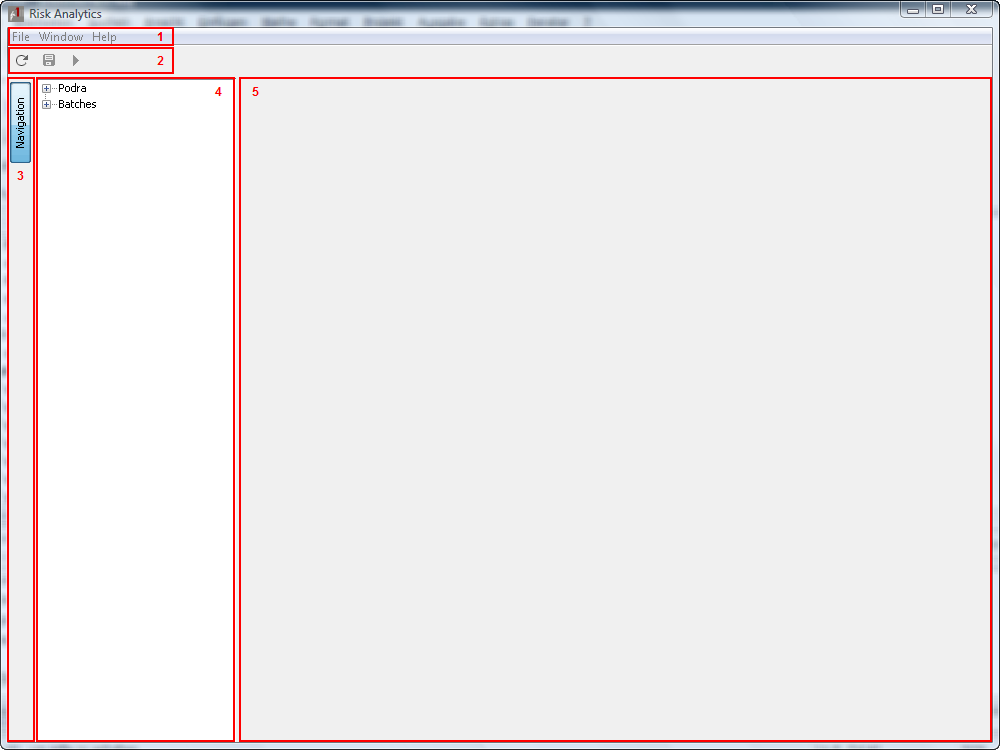
\includegraphics[scale=0.6]{images/UserInterfaceAreas.png}
	\caption{Areas of the user interface}
	\label{fig:UserInterfaceAreas}
\end{figure}


\section{Menu}
\label{sec:uiMenu}

\subsection{File menu}
\label{subsec:uiFileMenu}

The file menu (\cf Figure~\ref{fig:menuFile}) is used for all regards concerning parametrization files. 

\begin{figure}[htb]
	\centering
		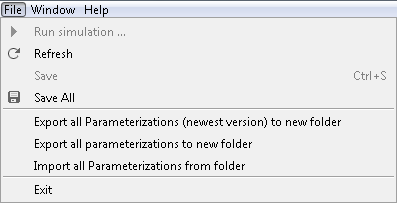
\includegraphics[scale=0.6]{images/menuFile.png}
	\caption{Expanded file menu.}
	\label{fig:menuFile}
\end{figure}

The following commands are available in this menu:
\begin{itemize}
\item \menu{Run simulation \ldots} As soon as a parameter file of any model is opened this command becomes available and starts the dialogue to run a simulation.
\item \menu{Refresh} reads the current state of the underlaying database and displays all stored model information in the navigation pane (\cf Section \ref{sec:uiNavigation}).
\item \menu{Save} When an open parametrization or result template is changed this command becomes enabled in order to save the current modifications. The standard shortcut \menu{STRG~+~S} can also be used instead.
\item \menu{Save All} works as the proir command except that it saves all modified parametrizations or result templates.
\item \menu{Export all Parametrizations (newest version) to folder} Since \RA{} can handle different versions of a parametrization this commant can be used for only exporting the latest version to a specified folder.
\item \menu{Export all Parametrizations to folder} In contrast to the previous function all versions of all parametrizations are exported here.
\item \menu{Import all Parametrizations from folder} This function can be used in order to import all parametrizations from a specified folder.
\end{itemize}

\subsection{Window menu}
\label{subsec:uiWindowMenu}

Without any data opened the \menu{Window} menu (\cf Figure~\ref{fig:menuWindow}) only contains the menu entry \menu{Settings} where the language of the user interface can be changed. 
If parametrizations, result templates or results are opened the according model is also listed in this menu. Since the data pane only shows data that belongs to one model this helps to keep track of the data that is currrently worked on if several models are involved.
\begin{figure}[htb]
	\centering
		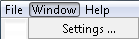
\includegraphics[scale=0.6]{images/menuWindow.png}
	\caption{Expanded window menu.}
	\label{fig:menuWindow}
\end{figure}

\subsection{Help menu}
\label{subsec:uiHelpMenu}

The menu \menu{Help} (\cf Figure~\ref{fig:menuHelp}) contains the entry \menu{About RiskAnalytics} where you can get information about the version, license, credits, used libraries and system properties.

\begin{figure}[htb]
	\centering
		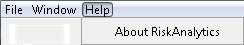
\includegraphics[scale=0.6]{images/menuHelp.png}
	\caption{Expanded help menu.}
	\label{fig:menuHelp}
\end{figure}

\section{Shortcuts}
\label{sec:uiShortcuts}

The shortcuts bar contains the most important functions of the \menu{File} menu namely
\begin{itemize}
\item \menu{Refresh}
\item \menu{Save}
\item \menu{Run Simulation \ldots}
\end{itemize}
The functions are explained in detail in Section~\ref{subsec:uiFileMenu}.

\section{Frame selection pane}
\label{sec:uiFrameSelection}

This part of the user interface helps hiding panes that are currently not needed in order to maximize the space on the screen for the relevant panes. In its initial state only the navigation pane (\cf Section~\ref{sec:uiNavigation}) can be hidden. When using data validation and comments on the data more options become available in this pane.

\section{Navigation pane}
\label{sec:uiNavigation}

In the navigation pane all the data processed in \RA{} is structured in a tree. The tree's top layer contains all available models (\eg \PODRA{}) as well as a node called \menu{Batches} that will be explained later in this section. The logical structure within all different models is identical thus, when expanding a model by pressing the plus sign next to its name, the following folders become visible:
\begin{itemize}
\item Parametrization
\item Result templates
\item Results
\end{itemize}

Since \RA{} is based on the data-driven-modelling paradigm a parametrization does not only contain pure data but also parts of the model structure itself. The model itself provides the components that generally can be proccessed during a simulation run such as \term{claims generators} or \term{underwriting segments}. The parametrization determines the number of the respective components as well as the actual numerical and type values of the components.

In contrast to the parametrization the result templates are structure-wise fully determined by the model itself. 

\subsection{Parametrization}
\label{subsec:parametrization}
When expanding the \menu{Parametrization} folder all parametrizations that are available for this model are listed at this place. In some cases a plus sign is visible next to the parametrization name. This indicates that different versions of a model are available. Right-clicking on the folder \menu{Parametrization} opens a context menu

\begin{figure}[htb]
	\centering
		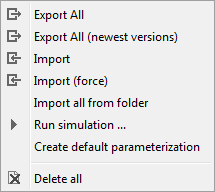
\includegraphics[scale=0.6]{images/menuParametrizationFolder.png}
	\caption{Context menu attached to the \menu{Parametrizations} folder.}
	\label{fig:menuParametrizationFolder}
\end{figure}

In following fuctions are available:
\begin{itemize}
\item \menu{Export All} \cf file menu.
\item \menu{Export All (newest versions)} \cf file menu.
\item \menu{Import} Select a parametrization file and import it into the database. If a parametrization is identical to a parametetrization that already exists in the database no new version is created.
\item \menu{Import (force)} Identical to the previous command except that the parametrization is imported at any case. If an identical parmanetrization already exists a new version with identical values is generated.
\item \menu{Import all from folder} This command imports all parametrization files from a specified directory into the respective model.
\item \menu{Run simulation} \cf file menu.
\item \menu{Create default parametrization} creates the empty default parametrization of the current model.
\item \menu{Delete all} deletes all parametrizations of the current model.
\end{itemize}

Some operations are only available for specific parametrizations. Thus, the options in the context menu slightly change when right-clicking a specific paramentrization (\cf Figure ~\ref{fig:menuParametrizationSingle}).

\begin{figure}[htb]
	\centering
		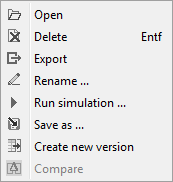
\includegraphics[scale=0.6]{images/menuParametrizationSingle.png}
	\caption{Context menu attached to a specific single parametrization.}
	\label{fig:menuParametrizationSingle}
\end{figure}

In following fuctions are available:
\begin{itemize}
\item \menu{Open} opens the paramerization in the data pane.
\item \menu{Delete} removes the selected parametrization from the database. Note that a parametrization can only be deleted if no result has already been generated with it. Other wise you will be asked if all results based on this parametrization should also be deleted.
\item \menu{Export} \cf file menu.
\item \menu{Rename} opens a dialogue in order to change the name of the parametrization and all depending versions.
\item \menu{Run simulation} \cf file menu.
\item \menu{Save as} saves the current parametrizations under a different parametrization name.
\item \menu{Create new version} If a specific version of the parametrization should be kept, a new version can be generated keeping the old on in its current state. If the user wants to open a used parametrization either it can be opened in read only mode or opened by generating a new version that is editable again.
\item \menu{Compare} If two or more parametrizations should be compared they can be selected using the CTRL key. Then the compare option becomes enabled. The lines in the parametrizations that differ in structure or in numerical values are highlighted.
\end{itemize}

\subsection{Result templates}
\label{subsec:resultTemplates}
The resulte template section is very similarly structured as the parametrizations section. Result templates are used in order to determine in dependently from a parametrization what results should be collected during the simulation and to what granularity. Result templates provide an easy way to get comparable results for different parametrizations. The use of templates guarantees that the same type of single result values are collected without having to specifying it again and again for different parametrizations.

All available options for dealing with result templates can be seen in Figure~\ref{fig:menuResultTemplateFolder} that shows the according context menu. The functions are analogous to the ones of parametrization that are described in Section~\ref{subsec:parametrization}.

\begin{figure}[htb]
	\centering
		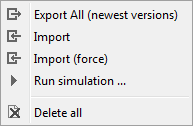
\includegraphics[scale=0.6]{images/menuResultTemplateFolder.png}
	\caption{Context menu attached to the \menu{Result templates} folder.}
	\label{fig:menuResultTemplateFolder}
\end{figure}

The functions that are available in the context menu for a specific result template are identical as the one for a parametrization thus we refer to Section~\ref{subsec:parametrization} for explanations.

\subsection{Results}
\label{subsec:results}

\section{Data pane}
\label{sec:uiDataPane}

